\documentclass[12pt]{article}
\usepackage{fullpage}
\usepackage[sc]{mathpazo} % Use the Palatino font
\usepackage[T1]{fontenc} % Use 8-bit encoding that has 256 glyphs
\linespread{1.75} % Line spacing - Palatino needs more space between lines

\usepackage{abstract}
\renewcommand{\abstractnamefont}{\normalfont\bfseries} % Set the "Abstract" text to bold
\renewcommand{\abstracttextfont}{\normalfont\small\itshape} % Set the abstract itself to small italic text


\usepackage{titlesec} % Allows customization of titles
\renewcommand\thesection{\Roman{section}} % Roman numerals for the sections
\renewcommand\thesubsection{\arabic{subsection}} % Roman numerals for subsections
\titleformat{\section}[block]{\large\scshape\centering}{\thesection.}{1em}{} % Change the look of the section titles
\titleformat{\subsection}[block]{\large}{\thesubsection.}{1em}{} % Change the look of the section titles

\usepackage{graphicx}
\graphicspath{ {images/} }


\title{\vspace{-15mm}\fontsize{24pt}{10pt}\selectfont\textbf{SVHN Classification}} % Article title
\author{
	\large
	\textsc{Team 'Les Mignonnes'}\\[2mm] % Your name
	\normalsize COMP 540 -- Machine Learning \\ % Your institution
	\normalsize Young Won Kim (yk41) -- Minh Pham (mnp7) % Your email address
	\vspace{-5mm}
}



\begin{document}
\maketitle

\hrulefill

\begin{abstract}
	\noindent Recognizing texts and digits from photographs has practical real world applications yet it is still a challenging computer vision problem. Machine learning, which utilizes statistical reasoning to approximate solutions for different problems, has been shown to accurately extract meaningful data from images. In this project, we attempted to classify images of house numbers from the Street View House Number dataset using different machine learning approaches. We were able to achieve high classification accuracy with neural network approaches, suggesting that these methods can capture crucial information from the images. 
\end{abstract}

\hrulefill

\section{Introduction}
\indent The Street View House Number (SVHN) is a real-world image dataset obtained from house numbers in Google Street View images. The images are of small cropped digits in RGB colors. Compared to MNIST, another well-known, widely used dataset, this is a harder, unsolved, real world problem, as it requires machines to learn and recognize digits in natural scene images. The dataset has been preprocessed (cropped) to only have one digit per image, and each image can be classified as one of ten classes. Digit '1' has label 1, '9' has label 9, and '0' has label 10. In total, there are 73257 images as a training set, 26032 images as test set, and 531131 addional images to use as extra training data. For technical reasons, we were not able to use the extra training data. Our goal was to correctly classify as many of the test images as possible. 

\indent We implemented new methods we had learned in class as semester progressed. First we started with non-neural network methods, namely k-nearest neighbor (KNN), one vs all (OVA) logistic regression, and softmax. Next, we moved on to built neural networks. Fully connected neural networks (FCN) and convolutional neural networks (CNN) all yielded higher test accuracy, although CNN performed slightly better. In building CNN, we used Tensorflow, an open source software library that is widely used for building deep neural networks. 

\indent Before choosing which algorithm to use, we visualized some of our training data. The images we get represent numbers [1, 9, 2, 3, 2, 5, 9, 3, 3, 1], and we confirmed that they are correctly labeled in the training set file (Figure 1). 

\begin{figure}[!tpb]
	\centerline{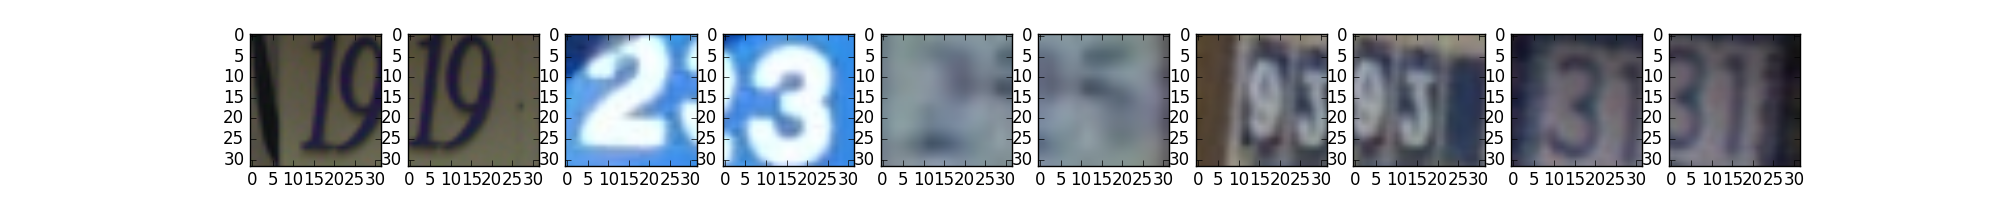
\includegraphics[width=80mm]{train_first10.png}}
	\caption{\label{Figure 1}
		First 10 images in the training set}
\end{figure}

\hrulefill

\section{Methods and Results}
\subsection{Resources}
Computational resources used for this project include MacBook Pros with 16G memory, desktops (Linux Ubuntu) with 32G memory, and a GPU that has 8G memory. 
\subsection{Data Pre-processing}

\begin{itemize}
	\item Grayscale\\
	Converting from RGB to grayscale would remove trivial features. We used a weighted method for grayscale conversion, which takes into account human perception of different colors (new grayscale image = (0.299 * R) + (0.587 * G) + (0.114 * B)).
	\item Normalization\\
	We also normalized pixel values in each image to be in the same range. Specifically, in each image, we subtracted the minimum pixel value and divided by the range of the pixel value (maximum - minimum).
	\item Validation data\\
	In order to tune different hyperparameters, we split the training set into ten and used one to be our validation set. Once we knew that our model was working, we used the whole training set for classifier algorithms to learn over when we making predictions on the test set.
	
\end{itemize}


\subsection{K-Nearest Neighbor}
\indent \indent We first used K-nearest neighbors (KNN) to learn over the training set and predict labels in the test set. Having performed 10-fold cross validation, we found that k = 15 gave best accuracy, with average accuracy being around 0.51 and relatively small standard deviation. With k = 15, the accuracy of our predictions came to be 0.49. We then converted RGB to grayscale, normalized the images and ran KNN. This resulted in a slight increase in test accuracy (at k=15), from 0.49 to 0.52. Moreover, normalizing the grayscale inputs in order to remove trivial features led to further increase in test accuracy (=0.53).

\subsection{One vs All}
\indent \indent Next, we tried OVA with different regularization terms (lambda). 
(more on OVA, why we expect it to succeed)
Lambda = 0, 1, and 50 all yielded prediction accuracy of 0.24, which is much lower than that of KNN 

\subsection{Softmax}
\indent \indent Softmax is a multi-class logistic regression classifier. It outputs normalized probabilities assigned to each label by minimizing the cross-entropy between the estimated class probabilities and the true distribution. 

 \indent When implementing Softmax on SVHN data, hyperparameter search gave us best validation accuracy of 0.23 with learning rate = 1e-7 and regularization = 5e+5 without normalization. With normalization, we achieved a higher best validation accuracy of 0.26 with learning rate = 5e-7 and regularization = 1e+5. This is consistent with achieving a higher accuracy by normalizing the images in KNN. However, the test accuracy was only 0.1.

\subsection{Fully Connected Neural Network}
\indent \indent We built a fully connected neural network, with 5 layers, each with 100 units. We converted the image date from RGB to YUV scale, since YUV color scheme is closer to human perception. We tuned a range of hyper-parameters for our neural network. We swept through batch size of 50 and 100; different update rules (ADAM, SGD, RMSPROP, and SGD with momentum); learning rates (1e-2, 1e-3, and 1e-4); weight scales (1e-2, 5e-2, 1e-3, and 1e-4). After 1 epoch, the best validation accuracy that we achieved was 63.7\% using batch size of 50, weight scale of 0.05, learning rate of 0.001, and ADAM update rule. We trained the whole training set to 20 epochs and we achieved a classification accuracy of 0.78. We also performed similar model on the RGB input and we achieved a classification accuracy of 0.73, suggesting that YUV conversion added some crucial features for classification.

\subsection{Convolutional Neural Network}
\indent \indent Our next logical step was to try CNN as it is known to perform well when the inputs are images. Regular neural networks do not scale well to larger images as they tend to result in a huge number of parameters, which then also leads to overfitting. In CNN, neurons in a layer will only be connected to a small region of the layer before it, instead of being fully connected.  Moreover, CNNs constrain the architecture in a way more suitable for images as inputs. The layers of CNN have neurons arranged in three dimensions - width, height, and depth. We can manipulate the final output layer to have dimensions 1x1x10 so that CNN architecture can reduce a full image into a single vector of scores for each classes. 


\indent Our first CNN consisted of two repeats of [Conv - ReLU - Pool] layers. The input images (32x32x3) were preprocessed by normalization and grayscale conversion, which flattens them to be (32x32x1). The first Conv layer has 32 filters with the size of 5x5 and stride = 1. Our second Conv layer has 64 filters with the size of 3x3 and stride = 1. Here, each image is zero padded automatically so that the output size will remain the same. ReLU layer applies an elementwise activation function of max(0,x). Pool layer carries out 2x2 max pooling. 

\indent After the two repeats of [Conv - ReLU - Pool] layers, we implemented one fully-connected layer. In order to prevent overfitting, we include a dropout method, which randomly drops units and their connections during training. Moreover, we use Adaptive Moment Estimation (ADAM) as our gradient descent algorithm. Lastly, our readout layer uses softmax as a loss function. Using this three-layered CNN allowed us to reach 0.88 as validation accuracy and 0.86 as test accuracy. In order to improve our accuracy, we tried various hyperparameter tuning. 

\begin{figure}[!tpb]
	\centerline{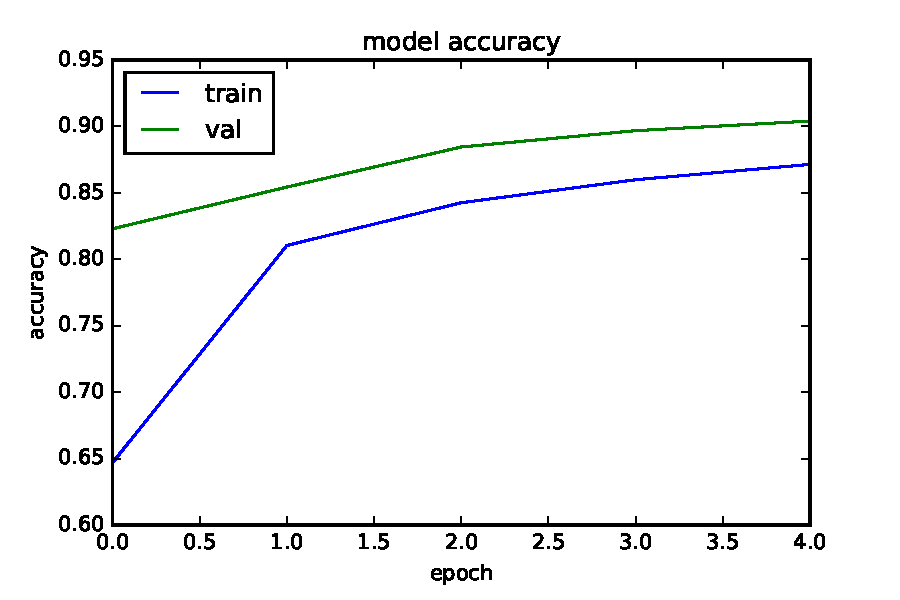
\includegraphics[width=80mm]{Accuracy_conv32_5x5_conv64_5x5_fc1024_all_dropout0_25.pdf}}
	\caption{\label{Figure 2}
		First CNN after implementing additional dropouts}
\end{figure}

\begin{figure}[!tpb]
	\centerline{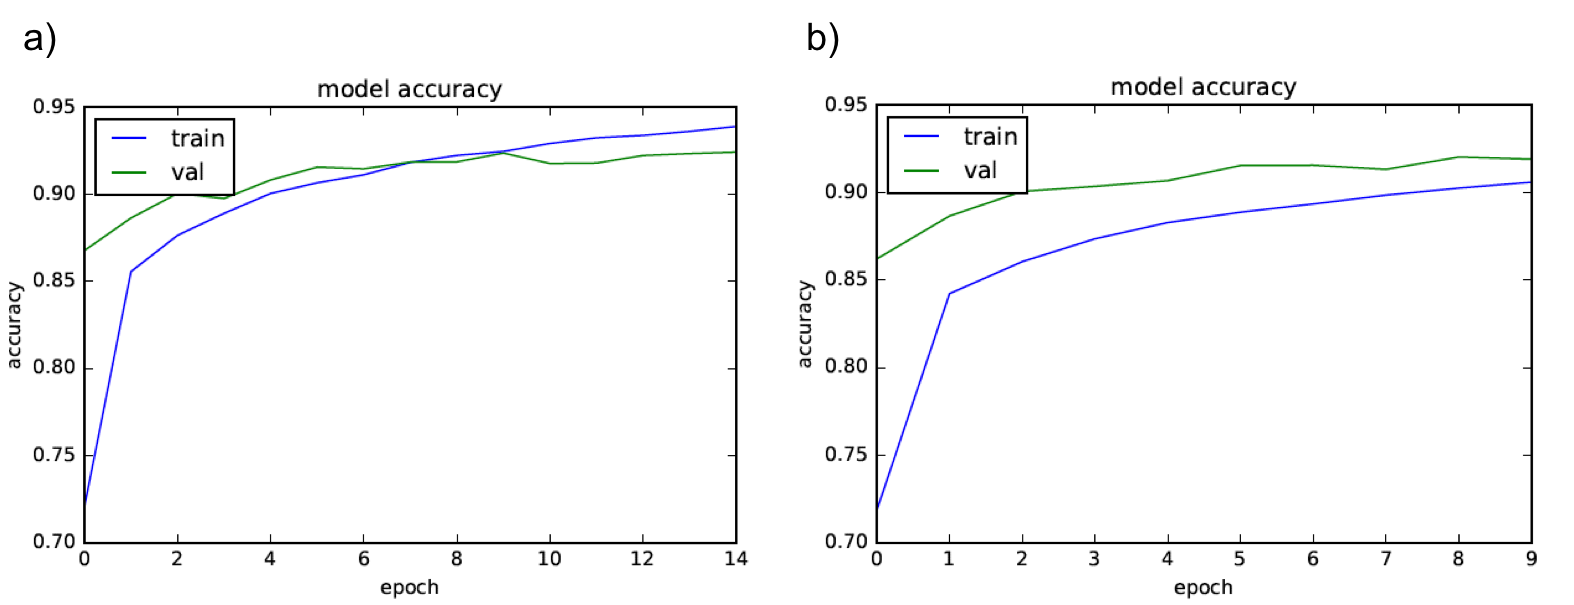
\includegraphics[width=80mm]{DropoutComparison.png}}
	\caption{\label{Figure 3}
		Using higher dropout probabilities results in less overfitting. a) Accuracy with dropout p = 0.5. b) Accuracy with dropout p = 0.25}
\end{figure}

\begin{figure}[!tpb]
	\centerline{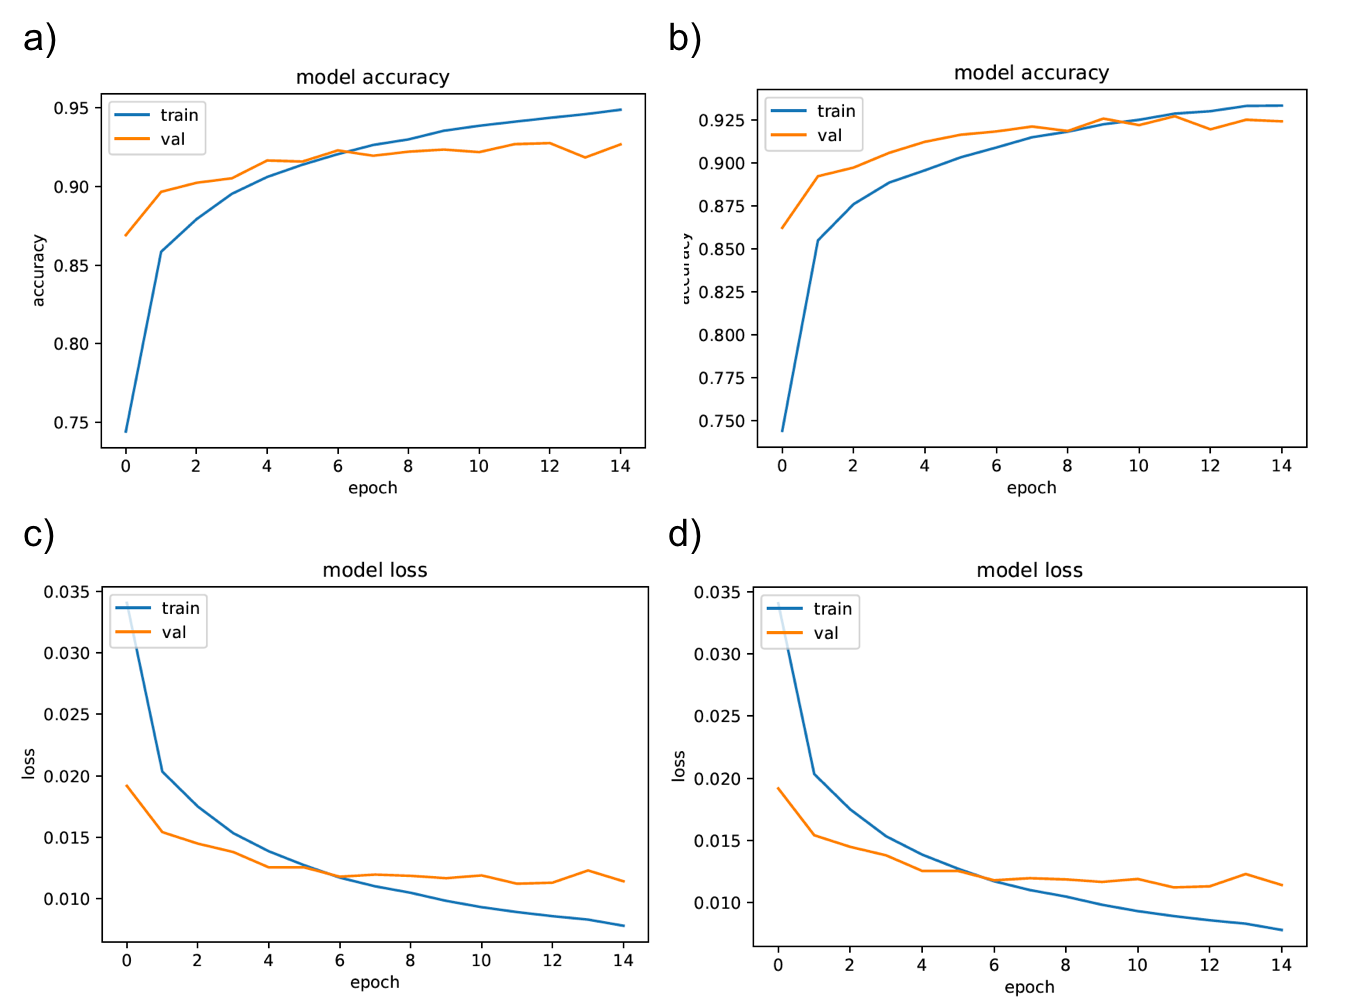
\includegraphics[width=80mm]{filtersizecomparison.png}}
	\caption{\label{Figure 4}
		Using smaller filter size results in higher accuracy and lower accuracy. a)Accuracy and c)loss of a model with two 3x3 filters. b)Accuracy and d)loss of a model with a 3x3 filter and 5x5 filter.}
\end{figure}

\begin{figure}[!tpb]
	\centerline{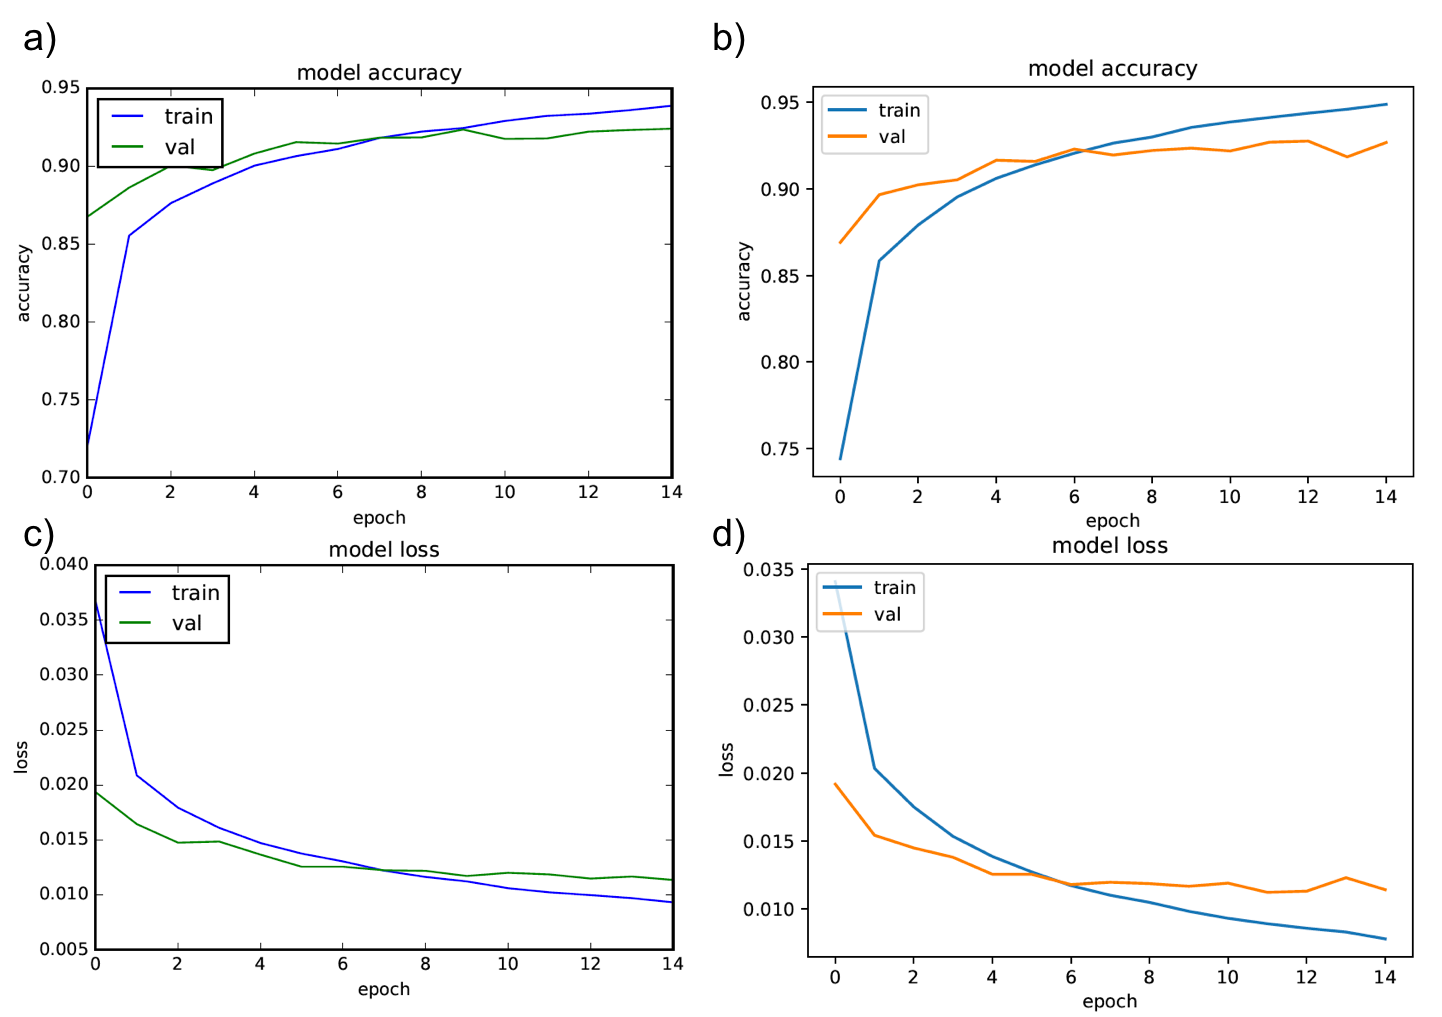
\includegraphics[width=80mm]{comparefcunits.png}}
	\caption{\label{Figure 5}
		Overfitting is observed faster in FC1024 than in FC512.a)Accuracy and c)loss of a model with FC1024. b)Accuracy and d)loss of a modell with FC512.}
\end{figure}

\begin{figure}[!tpb]
	\centerline{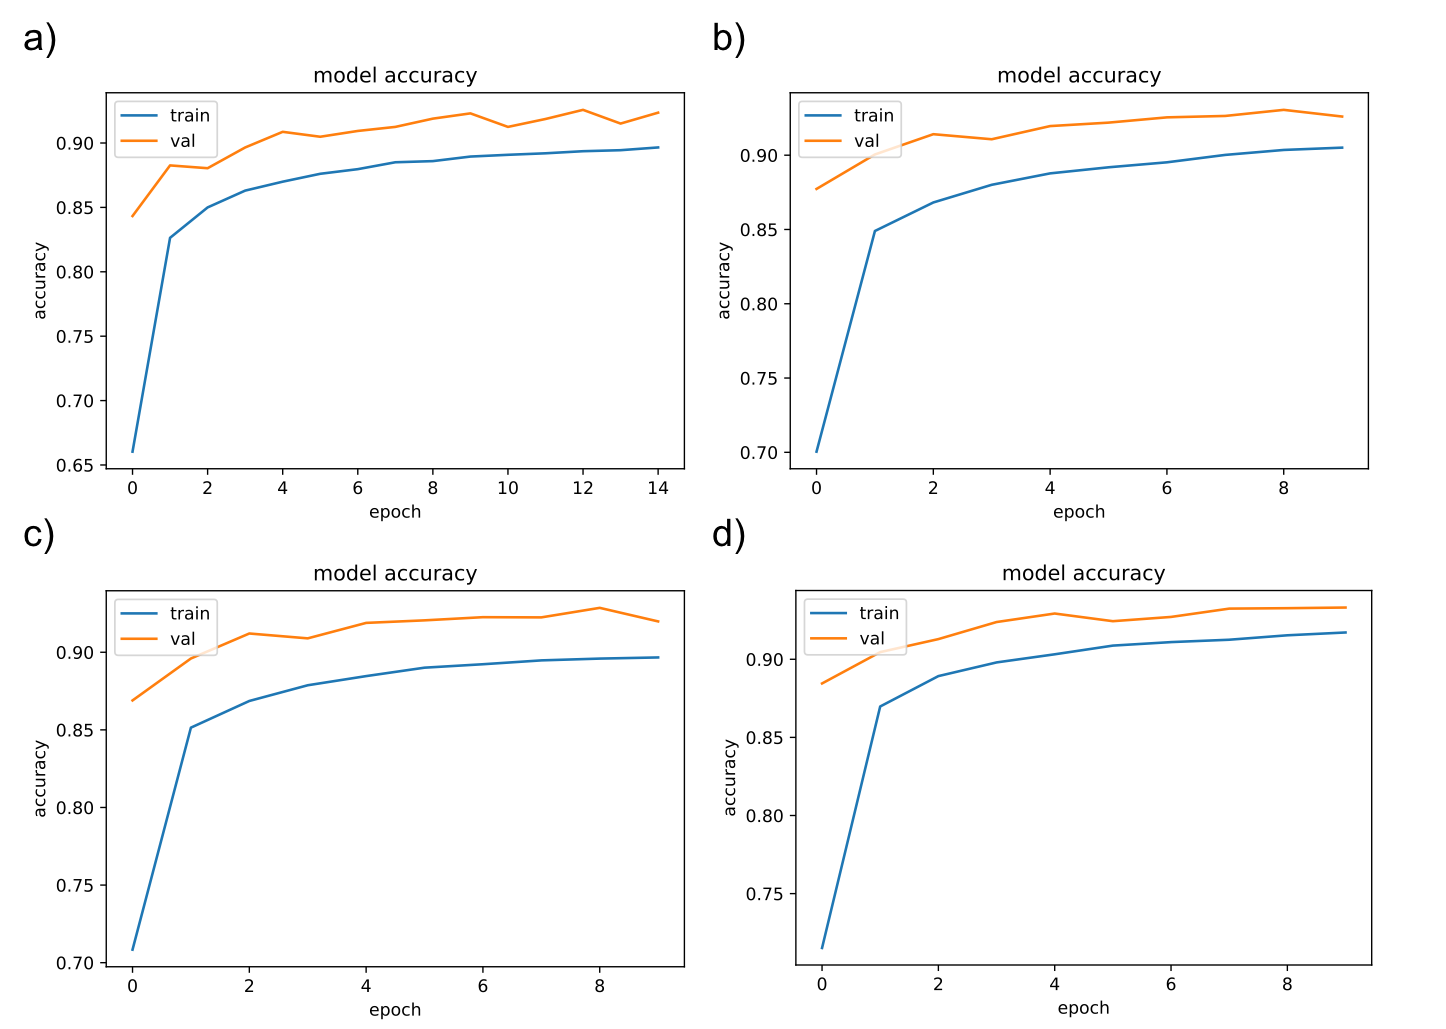
\includegraphics[width=80mm]{comparinglayerdepth.png}}
	\caption{\label{Figure 6}
		As we add more layers, accuracy converges faster. Accuracies with a) three conv layers (32,64,128), b) four conv layers (32,32,64,128), c) five conv layers (32,32,64,64,128) d) six conv layers (32,32,64,64,128,128)}
\end{figure}

\begin{figure}[!tpb]
	\centerline{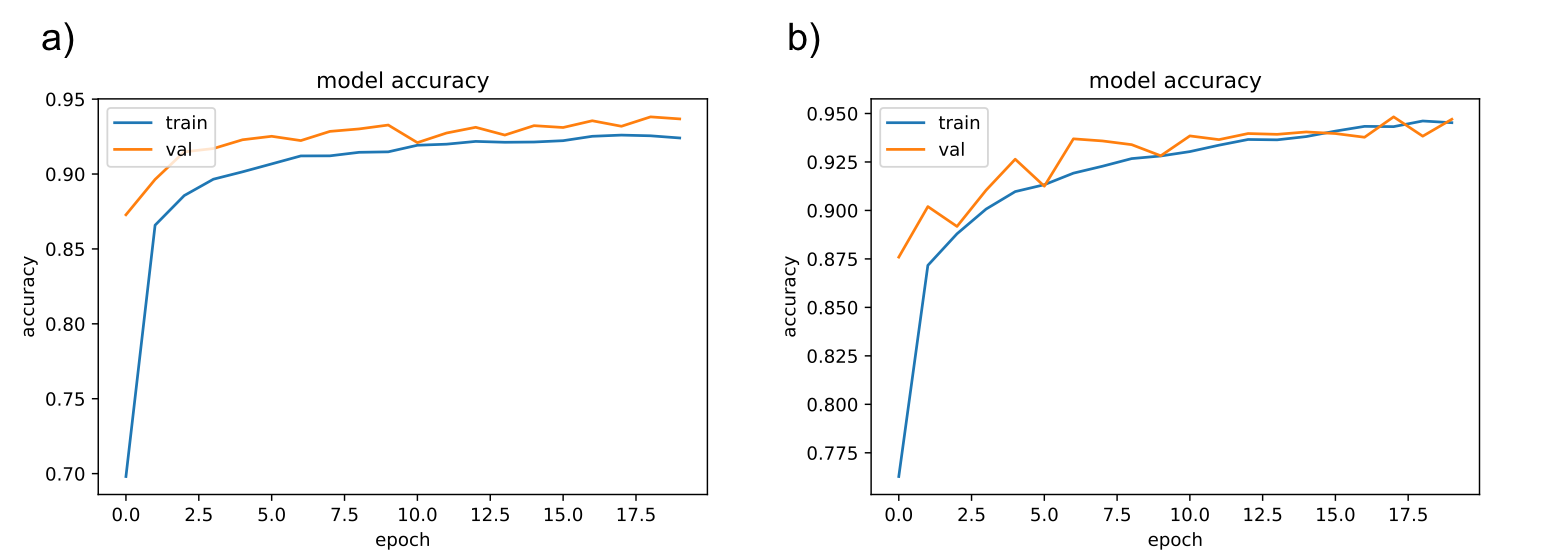
\includegraphics[width=80mm]{comparingbatchnorm.png}}
	\caption{\label{Figure 7}
		 Training accuracy with batch normalization converges faster, although validation accuracy in batch normalization does not increase as steadily as in non-batch normalization.}
\end{figure}

	\begin{itemize}
		\item Dropout\\
		From our first CNN, we observed that the training accuracy gets close to 1.0, which suggests that the model might be overfitting. To prevent this, we decided to introduce dropouts also after every two conv layers. In Figure 2, we see that our model is no longer overfitting. Moreover, using higher probabilities for droupout in FC layer results in less overfitting (Figure 3)
		
		\item Filter size\\
		We tuned our filter sizes to be either 3x3 or 5x5. With filter size 3, we achieve a higher overall accuracy much faster compared to when using filter size 5 (Figure 4). In addition, loss for filter size 3 converges faster than loss for filter size 5. 
		
		\item Number of units in FC layer\\
		Overfitting is observed faster in FC1024 than in FC512 (Figure 5). Train loss and accuracy overall are relatively similar. 
		
		\item Number of layers\\
		As we add more layers, accuracy and loss converge faster (Figure 6).
		
		\item Batch normalization\\
		To reduce the number of iterations for training, we decided to include batch normalization. Although validation accuracy in batch normalization does not increase as steadily as in non-batch normalization, we observed that training accuracy with batch normalization converges faster. For this reason we chose to include batch normalization for our final model (Figure 7).
				
		\item Gradient descent optimizers: ADAM, RMSprop, SGD\\
		Stochastic gradient descent (SGD) without or with momentum (momentum = 0.9) did not yield high overall accuracy as did ADAM model. RMSprop yielded relatively similar convergence of loss and accuracy and high overall accuracy like in Adam model. However, RMSprop did not yield a high test set accuracy. Based on such findings, and as ADAM method is also known to be most suitable method for neural network models, we chose ADAM as our gradient descent optimizer for our final model. 
		
		\item Learning rate for ADAM
		We tune learning rate for Adam as follow 0.01, 0.001, 0.0001. As the learning rate is too high (0.01), loss actually goes up and accuracy goes down as the number of epochs increases. Learning rates of 0.001 and 0.0001 yield similar converges in accuracy and loss. Overall accuracy is similar for the two learning rates. We decided to choose lr 0.001.  
	\end{itemize}

\indent Our final CNN consists of three repeats of [Conv - ReLU - Conv - ReLU - Pool] layers, resulting in six Conv layers. Before being put through layers, the input images (32x32x3) are preprocessed by normalization and grayscale conversion, which flattens them to be (32x32x1). The first two Conv layers each have 32 filters with the size of 3x3 and stride = 1. The next two Conv layers have 64 filters with the size of 3x3 and stride = 1. Our final two Conv layers have 128 filters with the size of 3x3 and stride = 1. At each Conv layer, images are zero padded automatically so that the output size will remain the same. After each Conv layer, ReLU layer applies an elementwise activation function of max(0,x), and batch normalization is performed. After each two Conv layers, pool layer carries out 2x2 max pooling, and we include a dropout method, which randomly drops units and their connections during training, in order to prevent overfitting.

\indent After the three repeats of [Conv - ReLU - Conv - ReLU - Pool] layers, we implement one fully-connected layer.  Moreover, we use Adaptive Moment Estimation (ADAM) as our gradient descent algorithm. Lastly, our readout layer uses softmax as a loss function. Using this seven-layered CNN allowed us to reach 95.3\% as test accuracy and rank 32 in Kaggle leaderboard. 


\begin{figure}[!tpb]
	\centerline{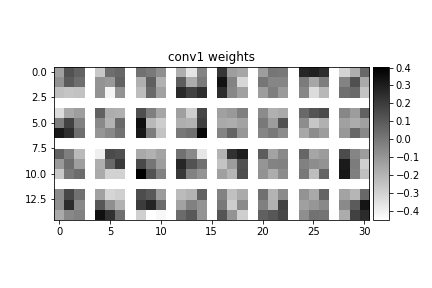
\includegraphics[width=80mm]{conv1_weights.png}}
	\caption{\label{Figure 8}
		Visualization of weights of the first Conv layer.}
\end{figure}

\begin{figure}[!tpb]
	\centerline{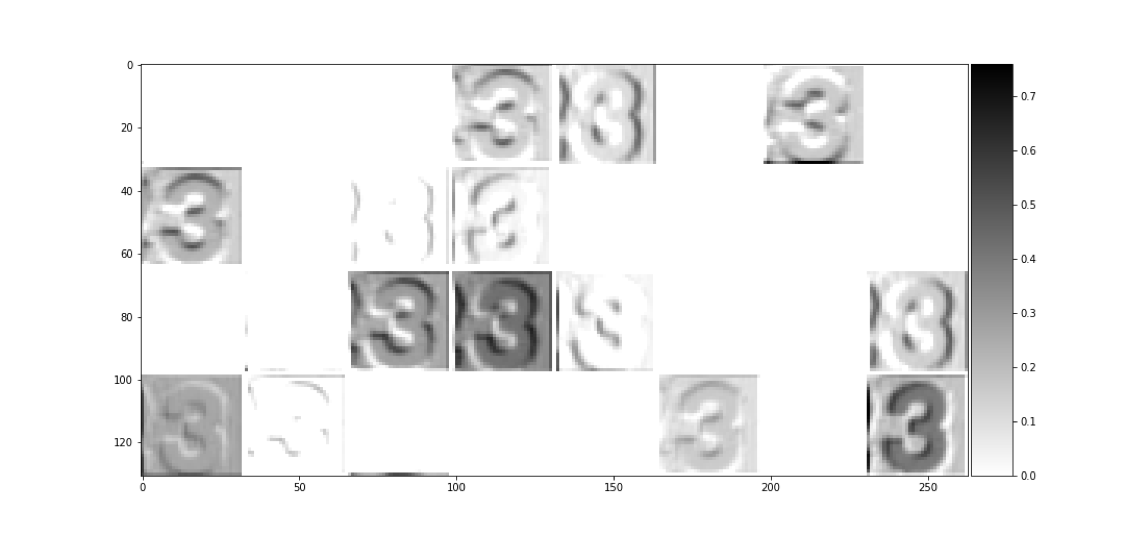
\includegraphics[width=80mm]{Conv1_Activate.png}}
	\caption{\label{Figure 9}
		Visualization of the first activation layer.}
\end{figure}

\begin{figure}[!tpb]
	\centerline{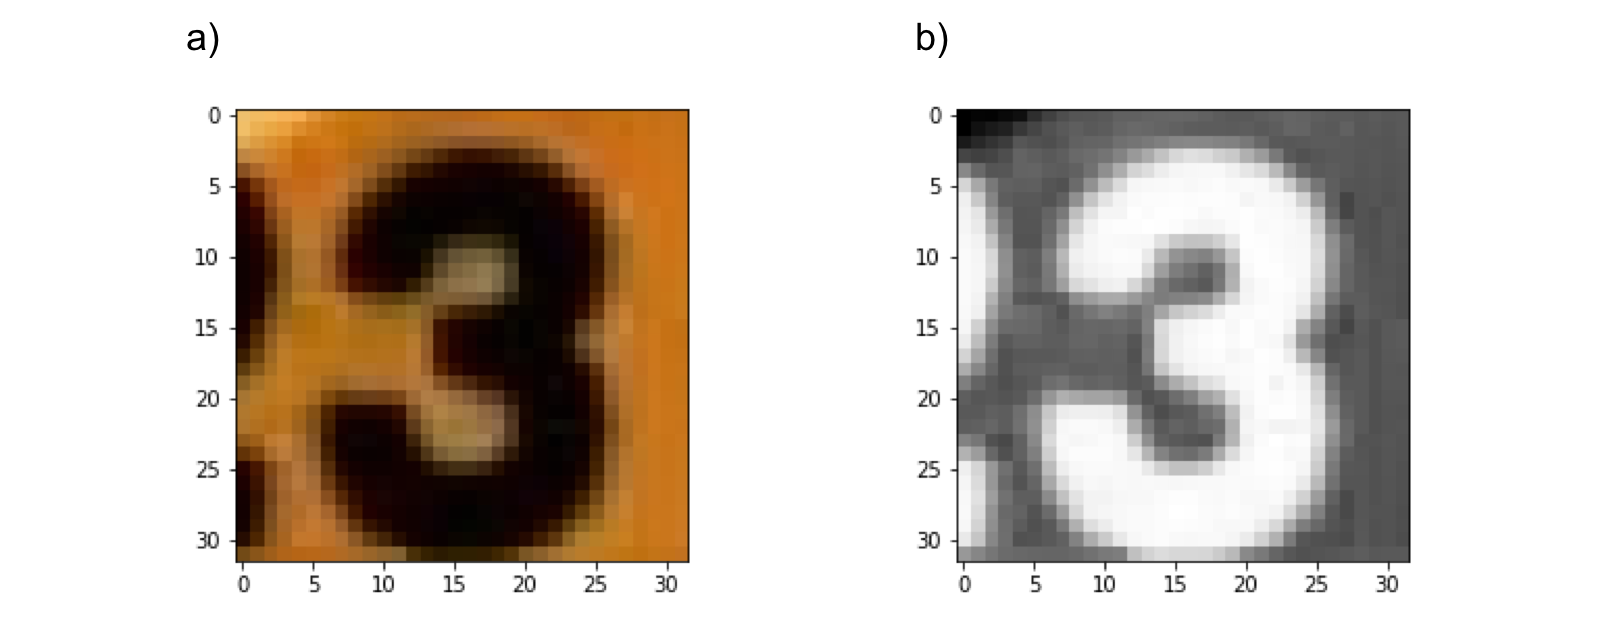
\includegraphics[width=80mm]{original.png}}
	\caption{\label{Figure 10}
		a) The original image of the fourth image in the training set. b) Grayscaled and normalized image of the fourth image in the training set.}
\end{figure}

\indent To look at what our final model learned, we visualized the weights in first Conv layer(Figure 8)]. Since the filter size is too small, it was difficult to recognize clear patterns. However, we were able to see some grayscale features cluster in the corners or middle parts of the filters. The features are relatively smooth, indicating a nicely converged network. We also visualized the first ReLU activation layer during the forward pass (Figure 9). The activations show features that are blobby and dense, accurately representing the original and grayscaled input image (Figure 10). These activation figures suggest that the first Conv layer can detect edges and pixel density of the digit in the image. Some activations are spare for many inputs, shown in white, suggesting that the learning rate might be a little bit high.

\hrulefill

\section{Discussion}

\begin{figure}[!tpb]
	\centerline{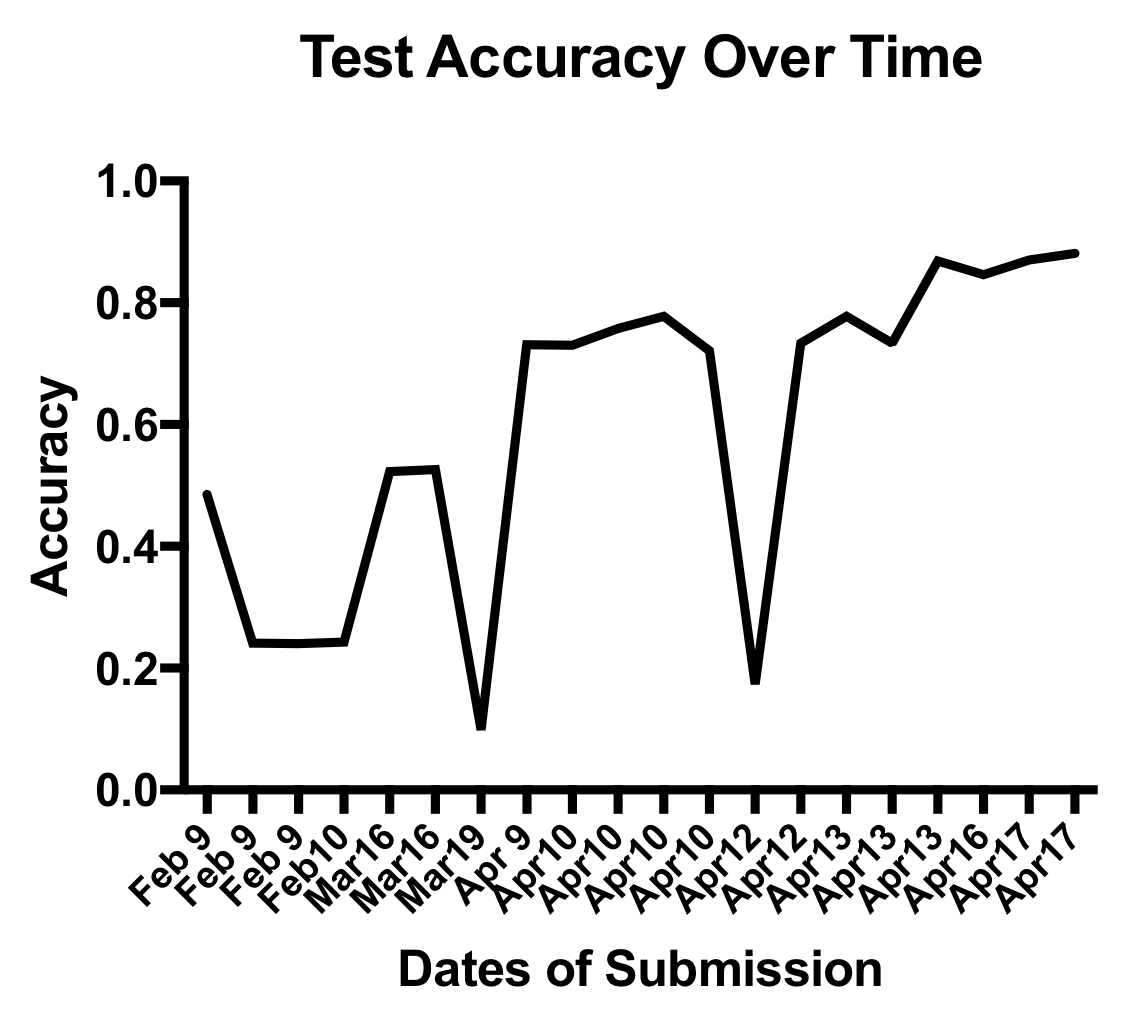
\includegraphics[width=80mm]{kagglesubmission.png}}
	\caption{\label{Figure 11}
		Kaggle submission accuracy over time}
\end{figure}


\indent \indent Throughout this project, we have implemented many different machine learning algorithms that we learned in class. We learned that especially for images, deep neural networks outperform non-neural network classifiers, and that choosing the architecture and hyperparameter tuning in neural networks are crucial for classification success. Figure 11 shows our test accuries over time. \\


\indent The state-of-the-art model [1], which achieved test accuracy of 99.31, combines max and average pooling and utilizes a tree-structured fusion of pooling filters. If we had more time, we could have used such methods to try and improve our accuracy. While our model achieves lower accuracy than a handful of popular, established methods, it does outperform one particular model that also uses different pooling methods and other multi-stage features [2]. They use what is called Lp pooling to improve their accuracy. However, we speculate that our model performs better because our network is deeper.

\indent One more thing we wanted to try but did not have the time to was using the extra dataset. We had seen that using more data as training set improves our accuracy and have tried to use the extra dataset. However, we did not have enough time to run our model using those data. We believe that we would have achieved a higher accuracy had we successfully used the extra dataset as part of our training data. 

\indent Our codes for neural network used TensorFlow initially, but we switched to Keras later. Using these open source libraries have made network building easier and faster.

\hrulefill
\section {References}
	1. Lee et al. Generalizing Pooling Functions in Convolutional Neural Networks: Mixed, Gated, and Tree, AISTATS, 2016\\
	2. Sermanet et al. Convolutional Neural Networks Applied to
	House Numbers Digit Classification, ICPR, 2012\\
\end{document}